\usetikzlibrary{arrows.meta,calc}
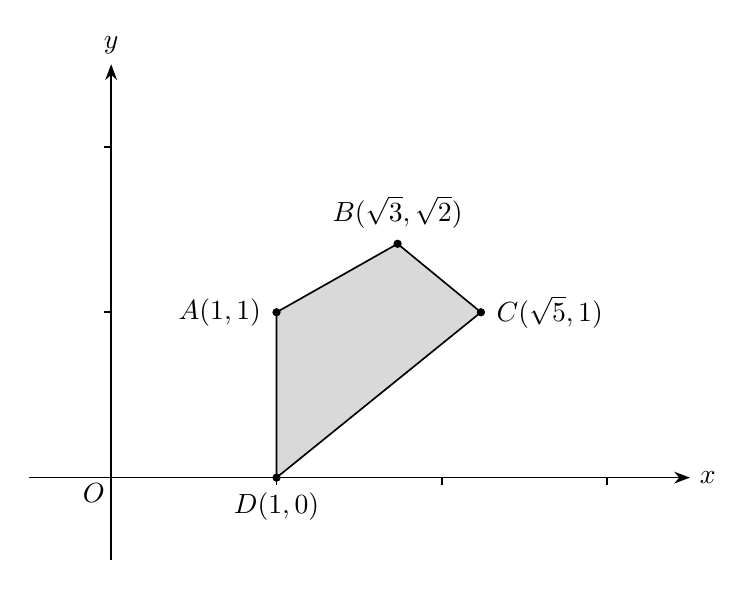
\begin{tikzpicture}[x=2.1cm,y=2.1cm,line width=.6pt,font=\normalsize,>=Stealth]
\coordinate (O) at (0,0);
\draw[->] (-0.5,0)--(3.5,0) node[right] {$x$};
\draw[->] (0,-0.5)--(0,2.5) node[above] {$y$};
\foreach \x in {1,2,3} {\draw (\x,0)--(\x,-0.045);}
\foreach \y in {1,2} {\draw (0,\y)--(-0.045,\y);}
\node[below left=2pt,inner sep=0pt] at (O) {$O$};

\coordinate (A) at (1,1);
\coordinate (B) at (1.7320508076,1.4142135624);
\coordinate (C) at (2.2360679775,1);
\coordinate (D) at (1,0);
\filldraw[fill=gray!30] (A)--(B)--(C)--(D)--cycle;
\fill (A) circle[radius=1.5pt];
\fill (B) circle[radius=1.5pt];
\fill (C) circle[radius=1.5pt];
\fill (D) circle[radius=1.5pt];
\node[anchor=east] at ([xshift=-2pt,yshift=0pt]A) {$A(1,1)$};
\node[anchor=south] at ([yshift=2pt]B) {$B(\sqrt{3},\sqrt{2})$};
\node[anchor=west] at ([xshift=2pt,yshift=0pt]C) {$C(\sqrt{5},1)$};
\node[anchor=north] at ([xshift=0pt,yshift=-2pt]D) {$D(1,0)$};
\end{tikzpicture}
